\documentclass[presentation]{beamer}
\usepackage{will-beamer-puebla} 
\tolerance=1000

\graphicspath{ 
  {figs/},
}

\setkeys{Gin}{width=\linewidth, height=0.85\textheight, keepaspectratio=true}

% \setbeameroption{show notes}

% \renewcommand\baselinestretch{1.2}

% \title[Ionized gas dynamics]{Dynamics of ionized gas around\\ massive young star clusters}
\title[Ionized gas dynamics]{Order versus disorder in\\ photo-ionized gas dynamics}
\author{\textit{William J. Henney}}
\date[Baltimore 2013]{
  December 2013 \(\cdot\) Puebla, Mexico
  \par\bigskip
  \alert{\textit{Remember to turn off power saver!}}
}

\institute[CRyA, UNAM]
{
  \structure{Centro de Radioastronomía y Astrofísica\\
    UNAM, Morelia, México}
}

\hypersetup{
  pdfkeywords={Massive Star Clusters, Astrophysics, Dynamics, Radiation},
  pdfsubject={},
  pdfcreator={Lovingly hand-crafted by the author using pdflatex and beamer}
}


\AtBeginSection[]
{
  \begin{frame}<beamer>
    \frametitle{Coming up next \dots}
    \tableofcontents[
    sectionstyle=show/shaded,
    currentsubsection, 
    hideothersubsections
    ]
  \end{frame}
}



\newcommand\missingmovietext{
  \begin{center}
    \bfseries\ttfamily
    This PDF viewer does not support embedded videos
    \par \bigskip
    To view the movie, please open the PDF file in \textit{Adobe Reader}
    
  \end{center}
  }

\begin{document}

\maketitle

\begin{frame}
\frametitle{Principal collaborators}
\par\medskip
\begin{columns}
  \column{0.75\linewidth}
  \begin{block}{CRyA-UNAM, Morelia, Mexico \dots}
    \begin{description}
    \item[\small HD] \textit{Jane Arthur}
    \item[\small Turbulence] \textit{Enrique Vázquez-Semadeni}
    \item \textit{Sac-Nicté Serrano Medina} (MSc)
    \item[\small Bowshocks] \textit{A. Jorge Tarango Yong} (MSc/PhD)
    \item \textit{Luis Ángel Gutierrez Soto} (MSc)
    \end{description}
  \end{block}
  \column{0.25\linewidth}
  \vspace*{-0.5cm}\par
  \hspace*{-1cm}\raisebox{0pt}[0pt][0pt]{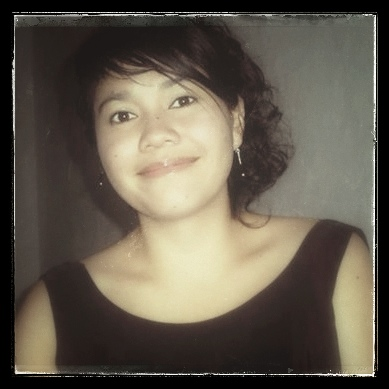
\includegraphics[width=2cm]{sac-fancy}}\\
  \hspace*{0.7cm}\raisebox{-1cm}[0pt][0pt]{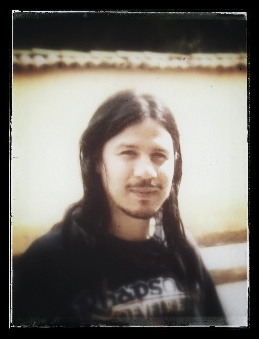
\includegraphics[width=2cm]{jorge-fancy}}\\
  \hspace*{-0.5cm}\raisebox{-2cm}[0pt][0pt]{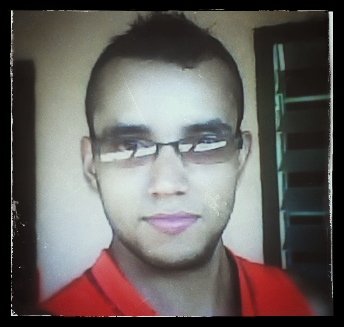
\includegraphics[width=2cm]{luis-fancy}}
  \hspace*{-2.5cm}\raisebox{0.3cm}[0pt][0pt]{\textit{\textbf{Students}}}
  \end{columns}

\begin{block}{Elsewhere in the world \dots}
  \begin{description}
  \item[\small MHD] \textit{Fabio de Colle} (ICN-UNAM, Mexico)
  \item[\small Radiation] \textit{Garrelt Mellema} (Stockholm Observatory, Sweden)
  \item[\small \textmu{}-physics] \textit{Gary Ferland} (Kentucky, USA)
  \item[\small Observations] \textit{María Teresa García-Díaz} (IA-UNAM, Ensenada, Mexico)
  \item \textit{Bob O'Dell} (Vanderbilt, USA)
    \end{description}
\end{block}

\end{frame}

\begin{frame}<beamer>
  \frametitle{Order versus disorder in photo-ionized gas dynamics}
  \tableofcontents[hidesubsections]
\end{frame}

\section{Part I: Disordered \hii{} regions?}
\subsection{Simulations}

\newlength\maxheight
\setlength\maxheight{0.8\textheight}
\newlength\moviewidth
\setlength\moviewidth{0.7\textwidth}
\newlength\movieheight

% \begin{frame}
% \frametitle{Turbulent models: initial conditions}
% \includegraphics{poland-figs/rgb-CPF-initial}
% \end{frame}

\begin{frame}
  \frametitle{Based on the following papers \dots}
  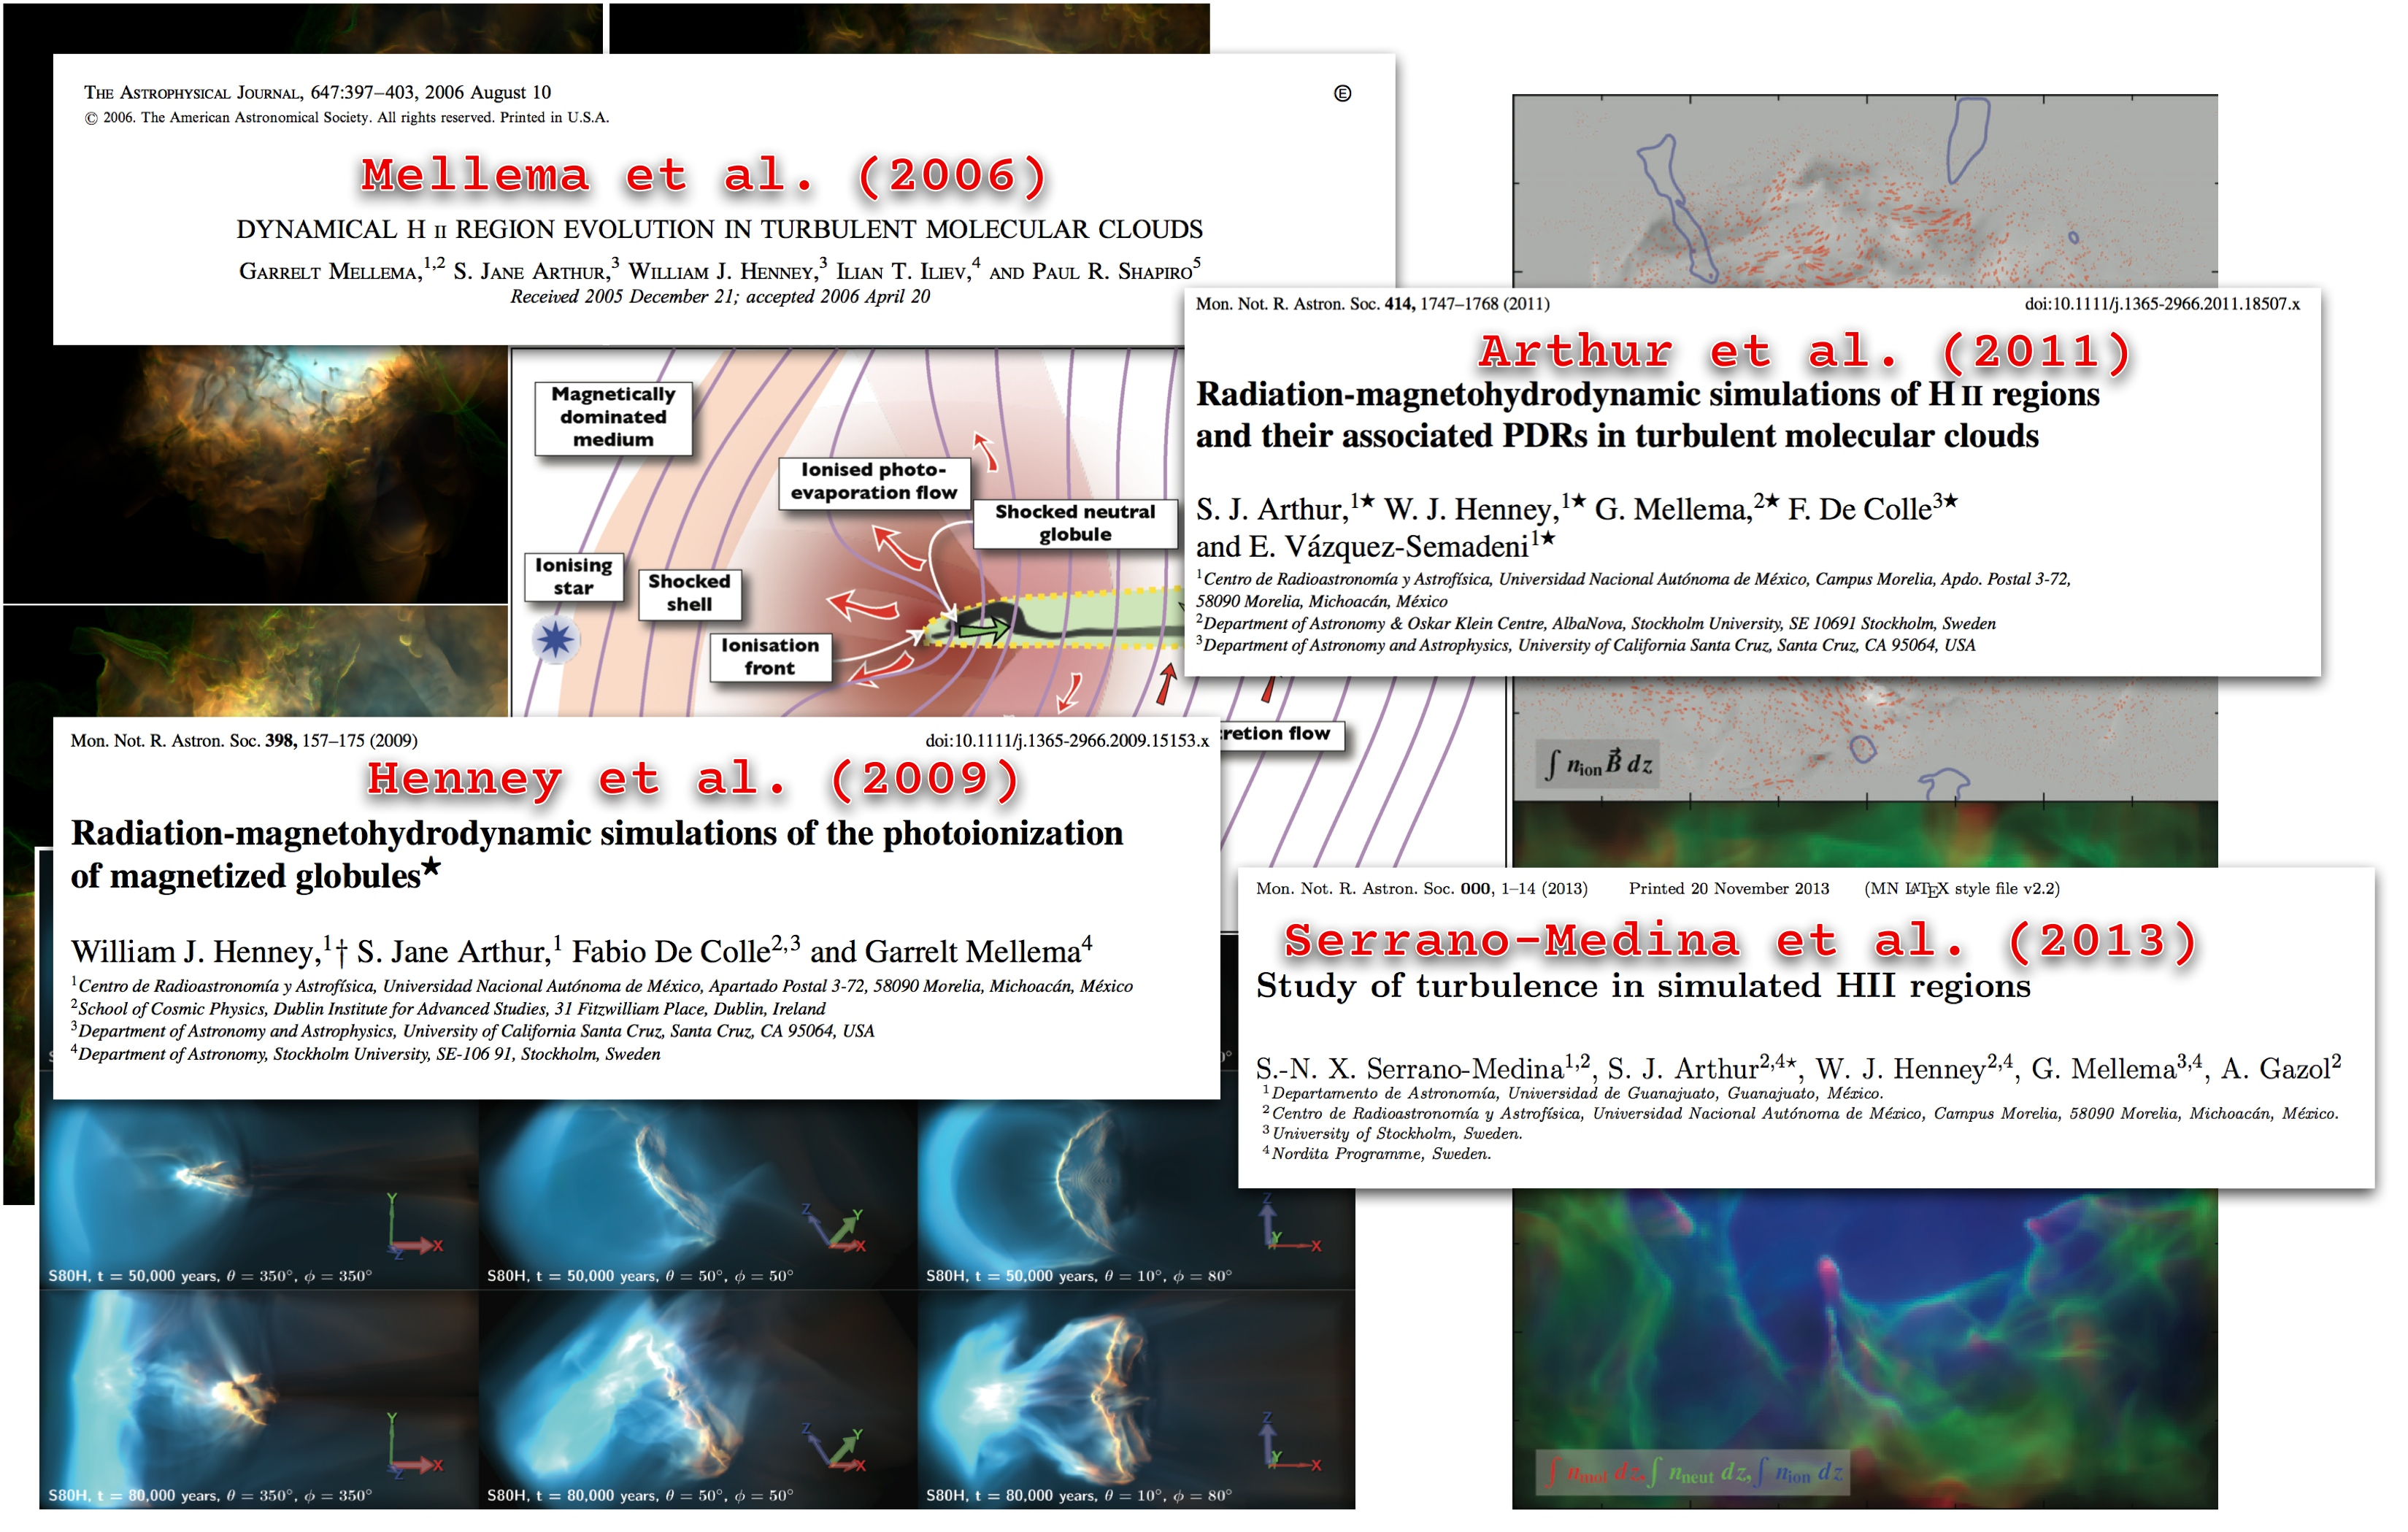
\includegraphics{Masthead-Multi}
\end{frame}
\begin{frame}[shrink=5]
\frametitle{Turbulent models: state of play}
\begin{block}{Physics we have}
  \begin{itemize}
  \item 3D time-dependent, hydrodynamics
  \item Approximate radiative transfer
  \item Microphysics:
    \begin{itemize}
    \item good for ionized gas
    \item fair for PDR
    \item poor for molecular gas
    \end{itemize}
  \item {}[Ideal magnetohydrodynamics]
  \end{itemize}
\end{block}
\begin{block}{Physics we lack}
  \begin{itemize}
  \item Stellar winds
  \item Radiation pressure
  \item Diffuse field
  \item Self-gravity
  \item{} 
    {\footnotesize Better microphysics, better radiative transfer,
    \scriptsize multifluids, non-ideal MHD, \tiny \(\upkappa\)-distributions, etc \dots}
  \end{itemize}
\end{block}
\end{frame}

% \begin{frame}[plain]%%
%   \newlength\figwidth
%   \setlength\figwidth{0.33\textwidth}
%   \renewcommand\arraystretch{0.0}
%   \setlength\tabcolsep{0pt}
%   \graphicspath{
%     {poland-figs/movie-stills/O-Star-512-PDR-2012/},
%     }
%   \begin{tabular}{lll}
%     \includegraphics[width=\figwidth]{01-Opening-Titles}
%     & 
%     \includegraphics[width=\figwidth]{02-Model-Parameters}
%     & 
%     \includegraphics[width=\figwidth]{03-Color-Scheme}
%     % & 
%     % \includegraphics[width=\figwidth]{04-Evolution-Start}
%     \\
%     \includegraphics[width=\figwidth]{05-Evolution-Mid}
%     & 
%     \includegraphics[width=\figwidth]{06-Evolution-End}
%     & 
%     \includegraphics[width=\figwidth]{07-Detail-View}
%     % & 
%     % \includegraphics[width=\figwidth]{08-Swimming-Sisters} 
%     \\
%     % \includegraphics[width=\figwidth]{09-Long-Wav-Color-Scheme}
%     % & 
%     \includegraphics[width=\figwidth]{10-Long-Wav-Mid}
%     & 
%     \includegraphics[width=\figwidth]{11-Long-Wav-End}
%     & 
%     \includegraphics[width=\figwidth]{12-Simulations-Credit}
% \end{tabular}

% \end{frame}


% This doesn't work with multimedia package since movie is opaque even
% in Preview.app
% \usebackgroundtemplate{
%   \parbox[c][\paperheight][c]{\paperwidth}{\missingmovietext}
% }

\def\MovieFile{poland-figs/O-Star-512-PDR-2012.mov}
% Ratio: 0.75
% \setlength\moviewidth{1.27968\paperheight}
% \setlength\movieheight{0.96\paperheight}
\begin{frame}%%
  \frametitle{Turbulent \hii{} regions: the movie\quad \small\texttt{youtube.com/divBequals0}}
  \graphicspath{
    {poland-figs/movie-stills/O-Star-512-PDR-2012/},
  }
  \begin{columns}
    %%
    %% The movie itself
    %%
    \column{0.7\linewidth}
    \setlength\moviewidth{\linewidth}
    \setlength\movieheight{0.75\moviewidth}
    \movie[width=\moviewidth, height=\movieheight, label=bigmovie,
    autostart, showcontrols, start=2s]
    {\includegraphics[width=\moviewidth, height=\movieheight]{01-Opening-Titles}}
    {\MovieFile}
    %%
    %% Buttons to control the movie
    %%
    \column{0.3\linewidth}
    \includegraphics[width=\linewidth]{02-Model-Parameters}
    \par\bigskip
    % Jump to Evolution
    \hyperlinkmovie[start=21s, duration=5s, loop]{bigmovie}
    {\beamerbutton{Evolution of optical line emission}}
    % Jump to 100,000
    \hyperlinkmovie[start=48s, duration=8s, palindrome]{bigmovie}
    {\beamerbutton{Rotation at \(t=100,000\)~years}}
    % Jump to 200,000
    \hyperlinkmovie[start=75s, duration=8s, palindrome]{bigmovie}
    {\beamerbutton{Rotation at \(t=200,000\)~years}}
    % Jump to Long wavelength
    \hyperlinkmovie[start=110s, duration=5s, loop]{bigmovie}
    {\beamerbutton{Neutral/molecular gas evolution}}
    % Jump to Credits 
    \hyperlinkmovie[start=153s]{bigmovie}
    {\beamerbutton{Show the credits}}
    % Open in viewer
    \href{run:\MovieFile}{\beamerbutton{Open in external viewer}}
  \end{columns}
\end{frame}

\subsection{Simulation results}

\begin{frame}
  \frametitle{Morphology and kinematics}
  \begin{columns}
    \column{0.55\linewidth}
    \begin{itemize}
    \item Many morphological features of observed \hii{} regions are
      reproduced naturally
      \begin{itemize}
      \item Due to existing density structure in the
        turbulent molecular cloud, combined with fragmentation induced
        by interaction with the ionized gas
      \end{itemize}
    \item Velocity dispersions of order the sound speed are
      maintained in the ionized gas during the entire evolution
    \end{itemize}
    \column{0.45\linewidth}
    \includegraphics[trim=0 190 0 0, clip, width=\linewidth]
    {poland-figs/comparison3_vs_t_Ostar}\\
    \includegraphics[trim=0 0 0 600, clip, width=\linewidth]{poland-figs/comparison3_vs_t_Ostar}
  \end{columns}
\end{frame}

\begin{frame}
  \frametitle{Energy equipartition (and lack thereof \dots)}
  \begin{columns}
    \column{0.5\linewidth}
    \begin{itemize}
    \item The highest pressure neutral and molecular gas is driven to
      near equipartition between thermal, magnetic, and turbulent energies
    \end{itemize}
    \smallskip
    \centering
    \includegraphics[height=0.6\textheight]
    {poland-figs/mhd-pressures-rgb-Ostar-et-0200-pram-pmag}\\
    \column{0.5\linewidth}
    \centering
    \includegraphics[height=0.6\textheight]
    {poland-figs/mhd-pressures-rgb-Ostar-et-0200-n-B}
    \begin{itemize}
    \item Lower pressure gas bifurcates into zones dominated by one or
      the other
    \end{itemize}
  \end{columns}
\end{frame}




\subsection{Observational diagnostics of ionized turbulence?}
\begin{frame}
  \frametitle{Evolution of simulated ``observed'' velocity statistics}
  \begin{block}{Second-order velocity structure function}
    \smallskip
    \centerline{\(
    S_2(l\,) = \sigma_{\mathrm{los}}^{-2}
    \left\langle 
      \left[ \widebar{V_{\mathrm{los}}} (\VEC{r}_1) 
        - \widebar{V_{\mathrm{los}}} (\VEC{r}_2) \right]^2 
    \right\rangle_{|\VEC{r}_1 - \VEC{r}_2| = l} 
    \)}
    \begin{itemize}
    \item Seems to steepen with time:
    \end{itemize}
    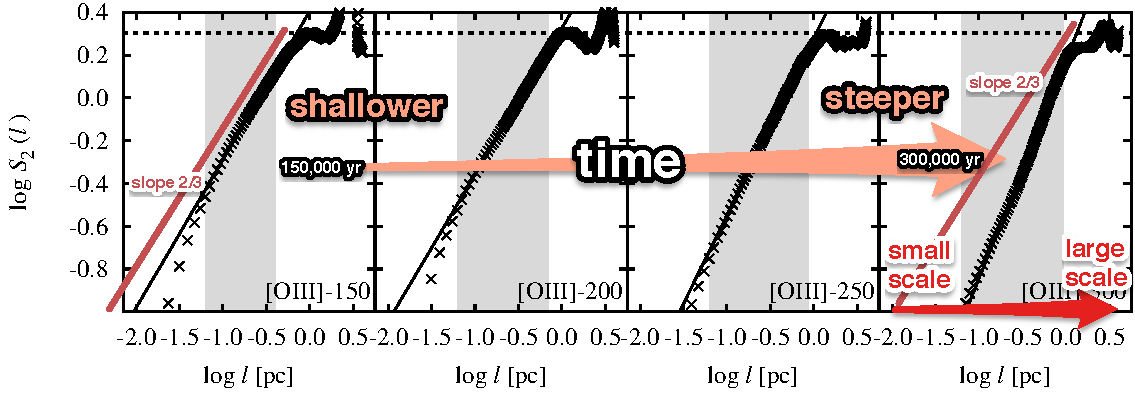
\includegraphics[width=\linewidth]{sf-will-oiii-annotate}
    \begin{itemize}
    \item Does this reflect an evolution of the underlying turbulence?
      \begin{itemize}
      \item Perhaps increasing compressibility?
      \item \textit{No} \dots it only occurs for certain viewing angles
      \end{itemize}
\end{itemize}
\end{block}

\end{frame}

\begin{frame}
  \frametitle{Champagne flows mess up the structure function}
  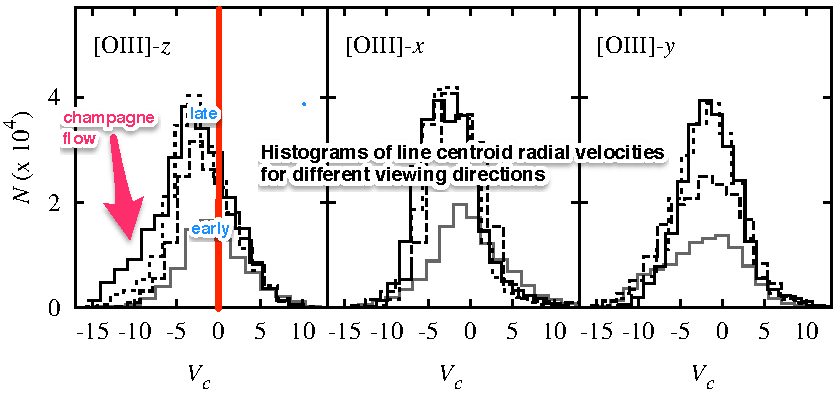
\includegraphics{pdf-vc-will-annotate}
  \begin{block}{Even over the so-called ``inertial'' range}
    
  \end{block}
\end{frame}

\begin{frame}
  \frametitle{But what about Velocity Channel Analysis?}
  \begin{itemize}
  \item Hopeless for H\(\upalpha\) -- more promising for [\ion{O}{3}]
  \end{itemize}
  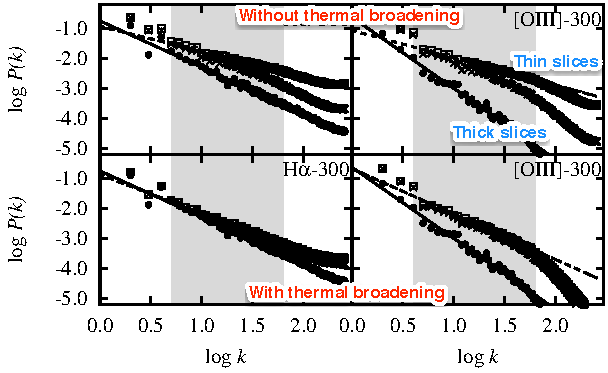
\includegraphics{vca-will-annotate}
\end{frame}

\subsection{Conclusions, part I}

\begin{frame}
  \frametitle{Conclusions to first part}
  \renewcommand\baselinestretch{1.5}\par
  \begin{itemize}
  \item \hii{} regions are turbulent (in simulations)
  \item This can explain observed non-thermal velocity widths
  \item Principal driver is density structure in the molecular cloud
    \begin{enumerate}
    \item Irregular champagne flow (early times)
    \item Overlapping photoevaporation flows (later times)
    \end{enumerate}
  \item Observational turbulence diagnostics are very tricky to apply
    \begin{itemize}
    \item (even to simulations)
    \end{itemize}
  \end{itemize}
\end{frame}


\section{Part II: Ordered \hii{} regions?}

\subsection{Kinematics and Proper Motions}
\begin{frame}
  \frametitle{Shortcomings of traditional kinematic probes}
  \begin{columns}
    \column{0.5\linewidth}
    \begin{block}{Spectroscopic radial velocities}
      \begin{itemize}
      \item Flows in only 1 dimension
      \item Limited by thermal broadening
      \end{itemize}
    \end{block}
    \column{0.5\linewidth}
    \begin{block}{Proper Motions}
      \begin{itemize}
      \item Non-steady flows only
      \item Requires sharp emission features
      \end{itemize}
    \end{block}
  \end{columns}
  \begin{block}{Is there another way?}
    \textbf{Yes!}
  \end{block}
\end{frame}

\subsection{Bowshocks as test particles}

\begin{frame}
  \frametitle{Stationary bowshocks as probes of the nebular flow}
  \includegraphics{balti-figs/LL1-schematic}
\end{frame}

\begin{frame}
  \frametitle{More bowshocks}
  \renewcommand\arraystretch{0}
  \setlength\tabcolsep{0pt}
  \begin{tabular}{l}
    \includegraphics[height=0.8\textheight]{balti-figs/north-west-field-combined}\\
  \end{tabular}%
  \begin{tabular}{l}
    \includegraphics[height=0.266\textheight]{balti-figs/LL266-558-15x15arcsec-annot}\\
    \includegraphics[height=0.266\textheight]{balti-figs/Proplyd-Bow2-10x10arcsec-annot}\\
    \includegraphics[height=0.266\textheight]{balti-figs/LL6-60x60arcsec-annot}\\
  \end{tabular}
\end{frame}

\begin{frame}
  \frametitle{Two-shock stationary flow pattern}
  \centering\includegraphics[width=\textwidth]{balti-figs/LL-outer-inner}
\end{frame}

\begin{frame}
  \frametitle{Types of flow interaction that give rise to bowshocks}
  \centering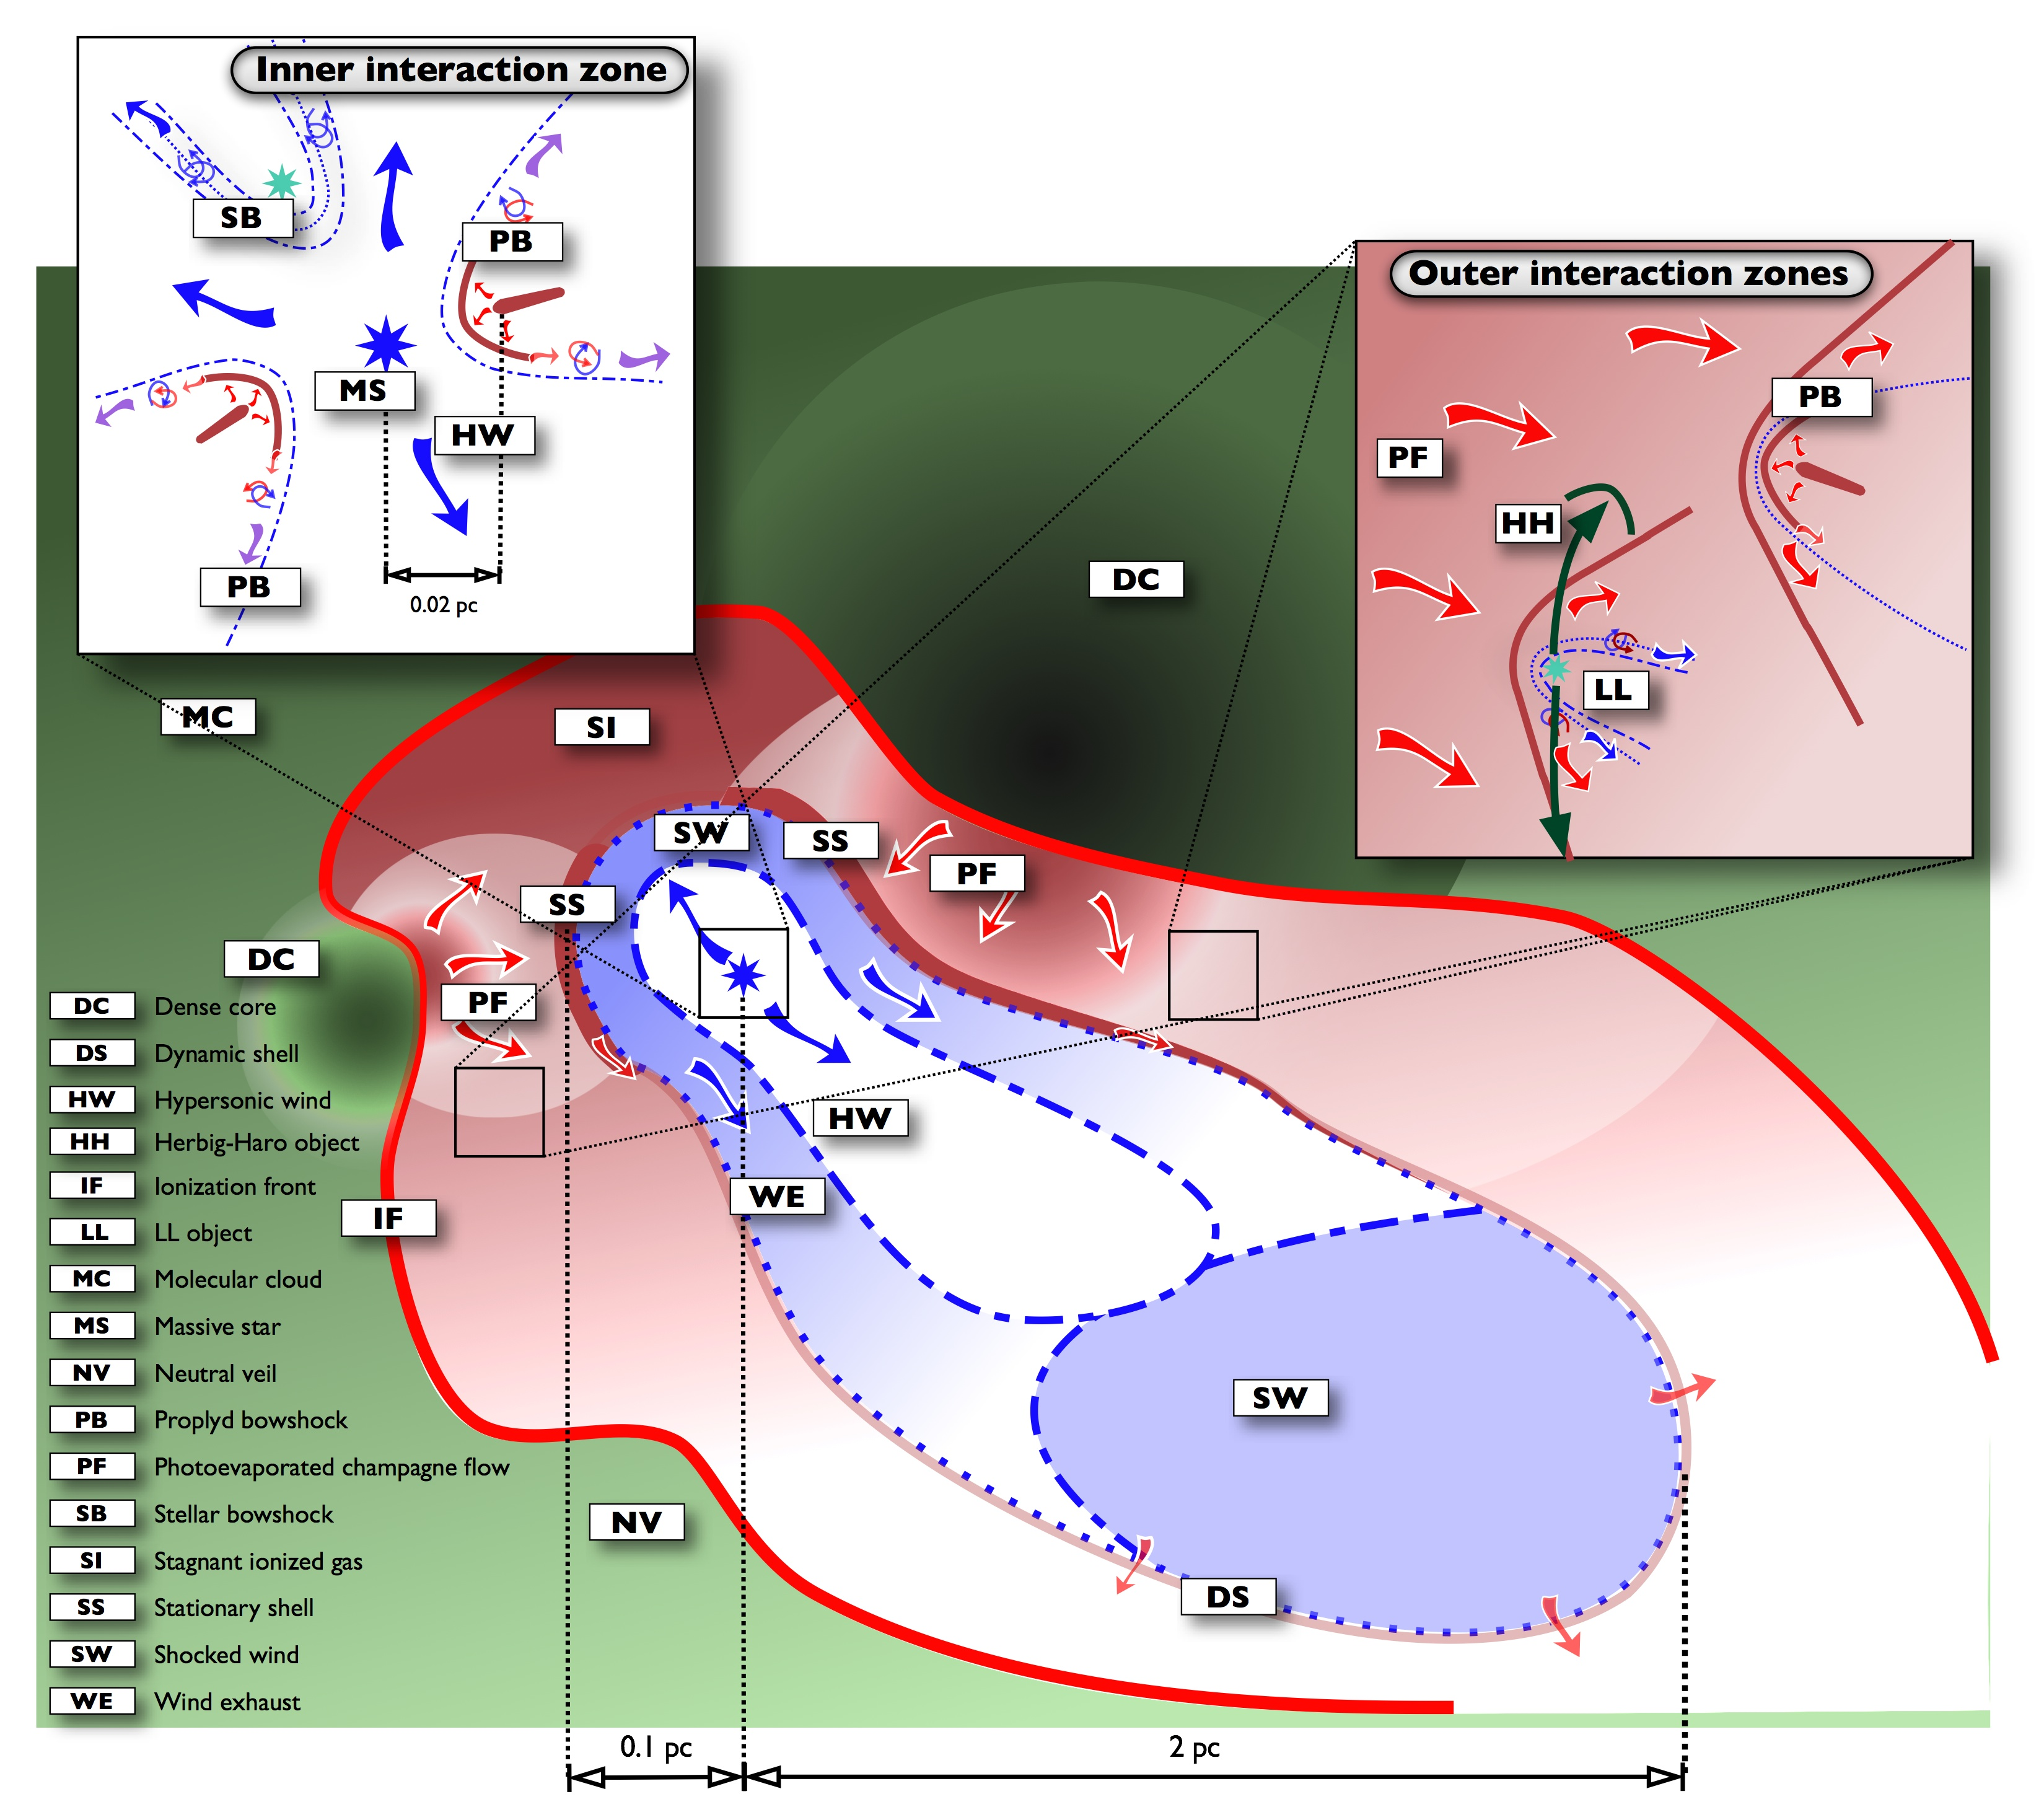
\includegraphics[width=\textwidth]{wind-geometry-extended}
\end{frame}

\subsection{Bowshock orientations}



\begin{frame}
  \frametitle{Orientation of the bowshocks in Orion}
  \centering
  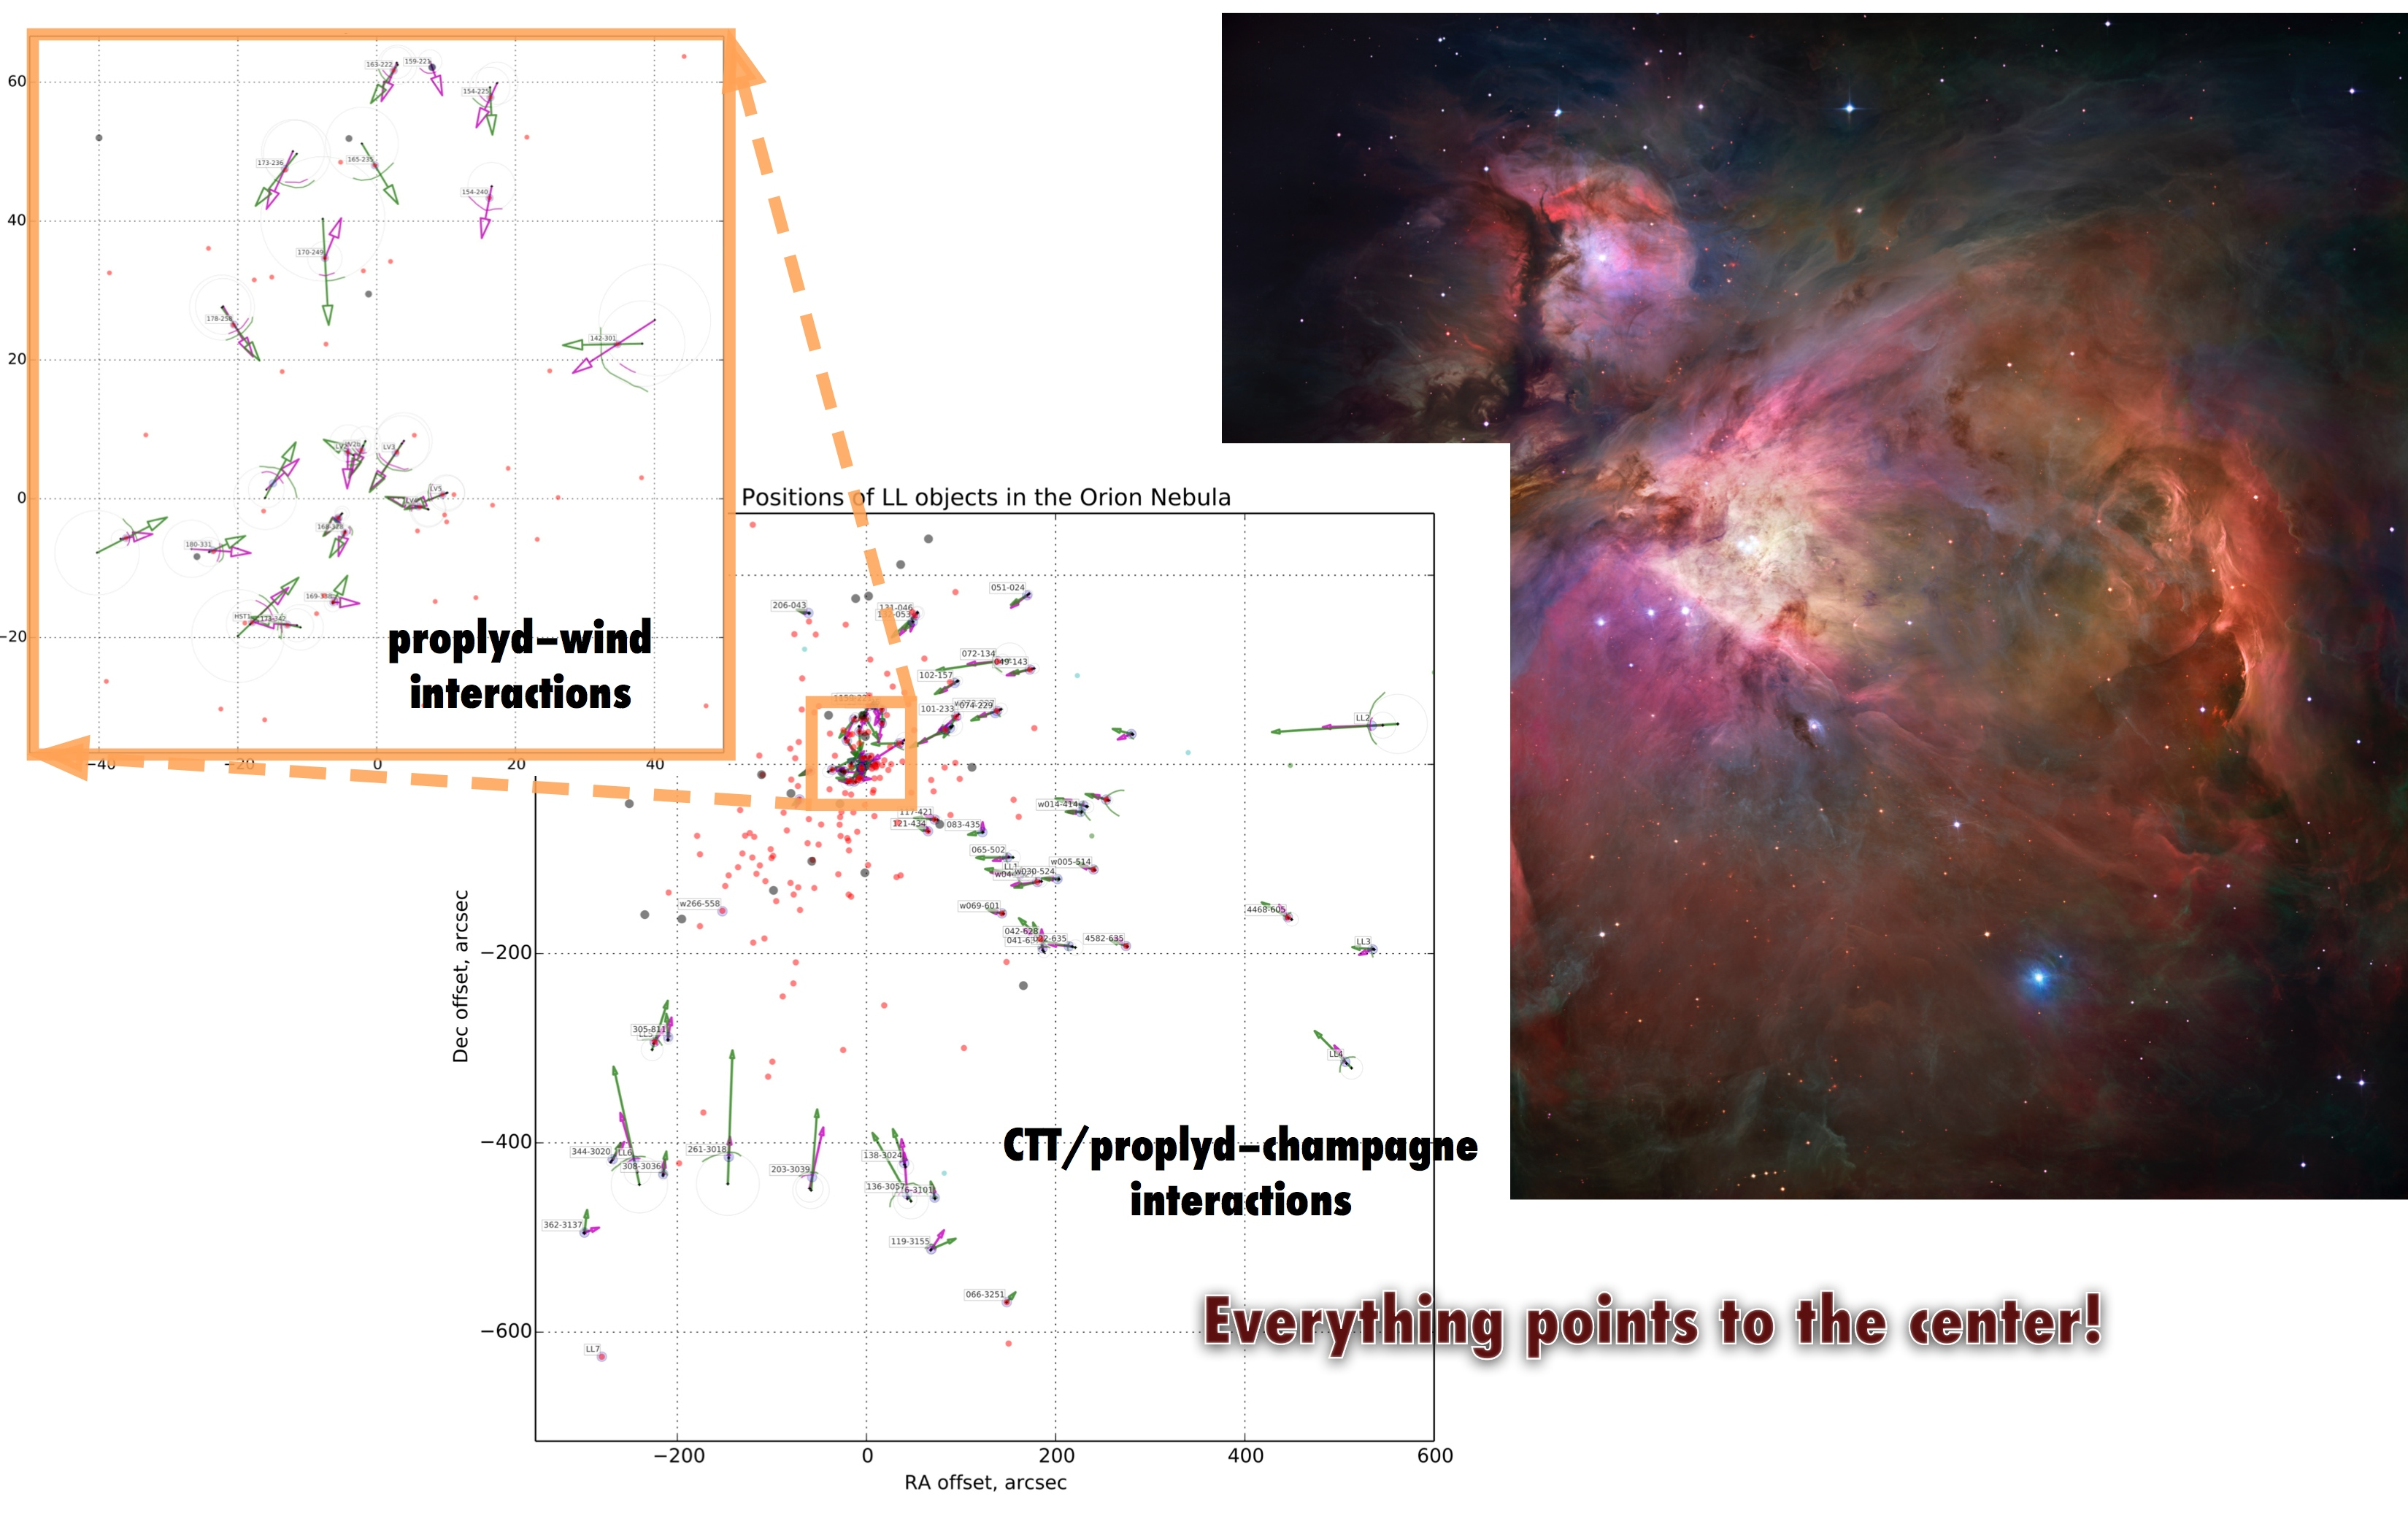
\includegraphics[width=\textwidth]{LL-Positions-Combo}
\end{frame}


\subsection{Conclusions, part II}

\begin{frame}
  \frametitle{Conclusions to second part}
  \begin{enumerate}
  \item Wind-wind bowshocks provide a promising \emph{third way} of
    probing the internal dynamics of \hii{} regions
    \begin{itemize}
    \item It is the \emph{only} way of measuring steady-state and/or
      smooth flows in the plane of the sky
    \item Local measure of the flow ram pressure and direction
    \item Can be applied to
      \begin{itemize}
      \item Proplyd--stellar-wind bowshocks (\(R < 0.1\)~pc)
        \Ref{Garc\'\i a-Arredondo et al.\ 2001}
      \item LL~Ori type bowshocks (\(R \simeq 0.1\)--\(1\)~pc)
        \Ref{Henney et al.\ 2013}
      \item OB-star bowshocks (\(R \sim 1\)~pc) \Ref{Povich et al.\ 2008}
      \end{itemize}

    \end{itemize}
  \item In Orion, bowshock orientation indicates an approximately
    ordered, radial flow
    \begin{itemize}
    \item In simulations, radially dominant flows are
      short-lived (\(\sim 10^5\)~years)
    \item Do we see Orion at a special time?
    \end{itemize}

  \end{enumerate}
\end{frame}

\end{document}
